\documentclass[border=1pt]{standalone}
\usepackage{tikz}
\usetikzlibrary{shapes.geometric, arrows}
\usepackage[default,osfigures,scale=0.95]{opensans}
\usepackage[T1]{fontenc}
\usepackage[utf8]{inputenc}


\tikzstyle{NormalBox} = [shape=rectangle, draw=blue, text=blue, thick, 
		align=center, fill=white, text width =2.5cm, minimum height=0.8cm,
		font=\bfseries ]
\tikzstyle{normalArrow} = [line width=0.05cm, ->, >=stealth, shorten >=0.3cm, shorten <=0.3cm]

\begin{document}
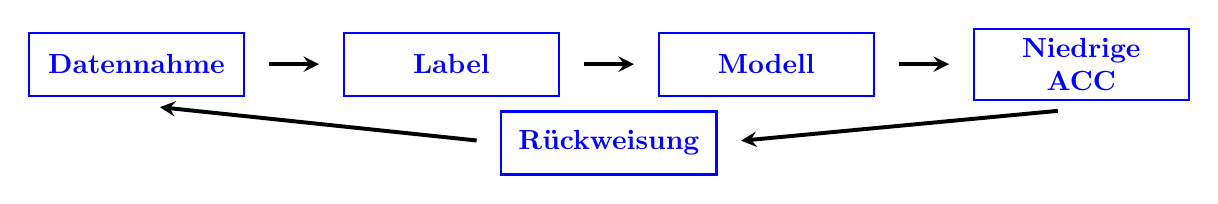
\begin{tikzpicture}[node distance=4cm]
    \node (A) [NormalBox] {Datennahme};
	\node (B) [NormalBox, right of=A]{Label};
	\node (C) [NormalBox, right of=B] {Modell};
	\node (D) [NormalBox, right of=C] {Niedrige ACC};
	\node (E) [NormalBox, below of=C, yshift=3.0cm, xshift=-2.0cm] {Rückweisung};
	\draw [normalArrow] (A) -- (B);
	\draw [normalArrow] (B) -- (C);
	\draw [normalArrow] (C) -- (D);
	\draw [normalArrow] ([yshift=-0.1cm]D.south) -- (E.east);
	\draw [normalArrow] (E.west) -- ([yshift=-0.1cm]A.south);
\end{tikzpicture}
\end{document}
